\section{Synchronization and Deadlocks}

\paragraph{Producer-Consumer Problem}
\begin{items}
  \item \textbf{Definition}: \\*
    $ - $ buffer is shared between producer and consumer (LIFO) \\*
    $ - $ \code{count} integer keeps track of number of currently available items \\*
    $ - $ producer produces item $ \to $ placed in buffer, \code{count++} \\*
    $ - $ buffer full $ \to $ producer needs to sleep until consumer consumed an item \\*
    $ - $ consumer consumes item $ \to $ remove item from buffer, \code{count--} \\*
    $ - $ buffer empty $ \to $ consumer needs to sleep until producer produces item
  \item \textbf{Problem}: \emph{race condition} on \code{count}
\end{items}

\paragraph{Producer-Consumer Problem --- condition variables}
\begin{items}
  \item \textbf{Solution}: can be solved with mutex + 2 counting semaphores \\*
    $ - $ hard to understand \\*
    $ - $ hard to get right \\*
    $ - $ hard to transfer to other problems
  \item \textbf{condition variables}: allow blocking until condition is met \\*
   $ - $ usually suitable for same problems but much easier to get right
  \item \textbf{Idea}: \\*
    $ - $ new operation performs \emph{unlock}, \emph{sleep}, \emph{lock} atomically \\*
    $ - $ new wake-up operation is called with lock held \\*
    $ \to $ simple mutex lock/unlock around CS + no signal loss
  \item \textbf{Pthread} condition variables: \\*
    $ - $ \code{pthread_cond_init}: create + initialize new CV \\*
    $ - $ \code{pthread_cond_destroy}: destroy + free existing CV \\*
    $ - $ \code{pthread_cond_wait}: block waiting for signal \\*
    $ - $ \code{pthread_cond_timedwait}: block waiting for signal or timer \\*
    $ - $ \code{pthread_cond_signal} : signal another thread to wake up \\*
    $ - $ \code{pthread_cond_broadcast}: signal all threads to wake up
\end{items}
\begin{figure}[H]\centering\label{ConditionVariables}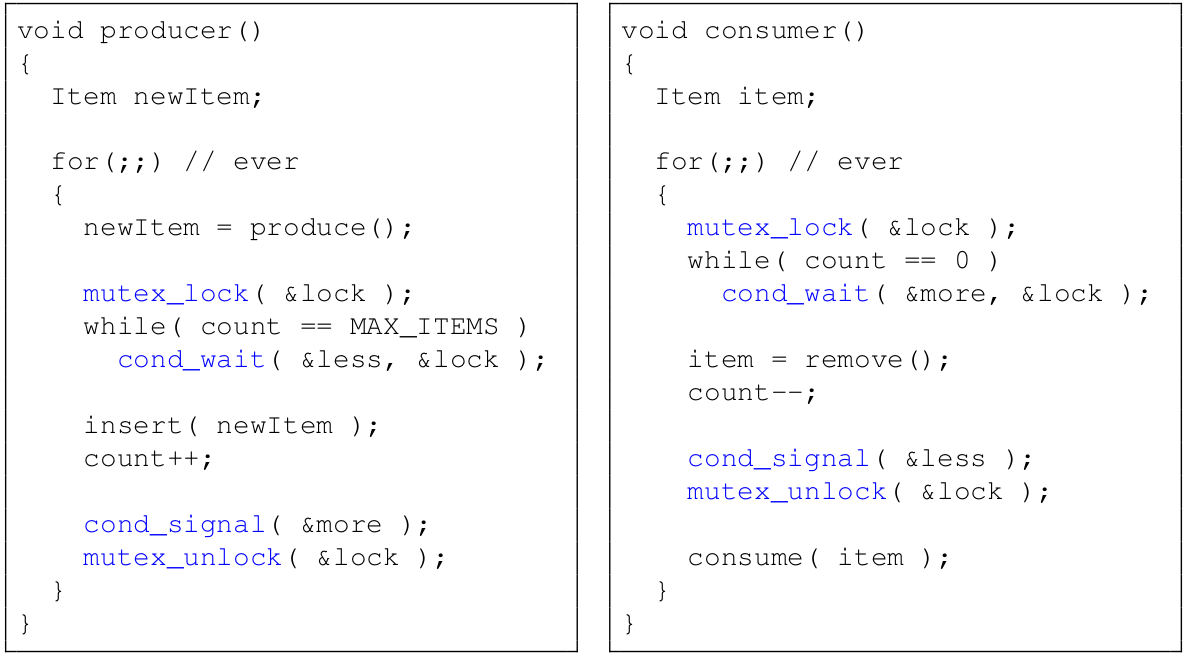
\includegraphics[width=0.33\textwidth]{ConditionVariables}\end{figure}

\paragraph{Reader-Writer Problem}
\begin{items}
  \item \textbf{Problem}: model access to shared data structures \\*
    $ - $ many threads compete to read/write same data \\*
    $ - $ \emph{readers}: only read data set, not performing any updates \\*
    $ - $ \emph{writers}: both read and write \\*
    $ \leadsto $ using single mutex for read/write operations is not a good solution! \\*
    \phantom{$ \leadsto $} (unnecessarily blocking out multiple readers while no writer is present)
  \item \textbf{Idea}: locking should reflect different semantics for reading/writing \\*
  $ - $ no writing thread $ \to $ multiple readers may be present \\*
  $ - $ writing thread $ \to $ no other reader/writer allowed
\end{items}

\paragraph{Dining-Philosophers Problem}
\begin{items}
  \item \textbf{Definition}: 5 philosophers with cyclic workflow: \\*
    $ - $ think \\*
    $ - $ get hungry \\*
    $ - $ grab one chopstick \\*
    $ - $ grab other chopstick \\*
    $ - $ eat \\*
    $ - $ put down chopsticks
  \item \textbf{Rules}: \\*
    $ - $ no communication \\*
    $ - $ no atomic grabbing of both chopsticks \\*
    $ - $ no wrestling
  \item \textbf{Abstraction}: models threads competing for limited number of resources
  \textbf{Problem}: what happens if all philosophers grab left chopstick at once?
  \item \textbf{Deadlock workarounds}:  \\*
    $ - $ just 4 philosophers allowed at table of 5 $ \to $ \emph{deadlock avoidance} \\*
    $ - $ odd philosophers take left chopstick first, even ones take right first $ \to $ \emph{deadlock prevention}
\end{items}
\begin{figure}[H]\centering\label{DiningPhilosophers}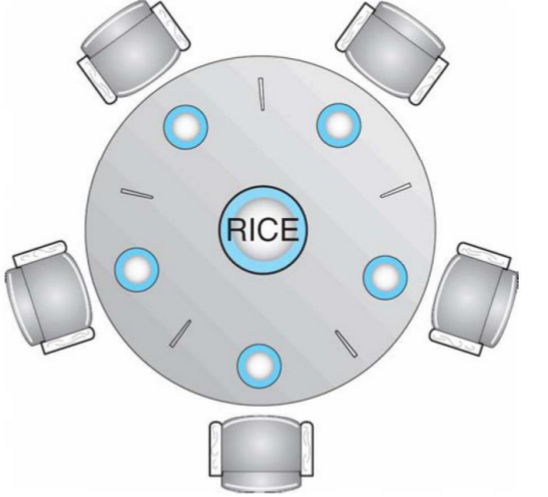
\includegraphics[width=0.2\textwidth]{DiningPhilosophers}\end{figure}

\paragraph{Deadlocks}
\begin{items}
  \item \textbf{Deadlocks} can arise if all four conditions hold simultaneously: \\*
    $ - $ \emph{mutual exclusion}: limited resource access (can only be shared with finite number of users) \\*
    $ - $ \emph{hold and wait}: wait for next resource while already holding at least one \\*
    $ - $ \emph{no preemption}: granted resource cannot be taken away but only handled back voluntarily \\*
    $ - $ \emph{circular wait}: possibility of circularity in requests graph
\end{items}

\paragraph{Deadlocks --- countermeasures}
\begin{items}
  \item \textbf{prevention}: pro-active, make deadlocks impossible to occur
  \item \textbf{avoidance}: decide on allowed actions based on a-priori knowledge
  \item \textbf{detection} (\emph{recovery}): react after deadlock happened
\end{items}

\paragraph{Deadlocks --- prevention}
\begin{items}
  \item \textbf{Goal}: negate at least one of the required deadlock conditions: \\*
    $ - $ \emph{mutual exclusion}: buy more resources, split into pieces, virtualize \\*
    $ - $ \emph{hold and wait}: get all resources en-bloque, 2-phase-locking \\*
    $ - $ \emph{no preemption}: virtualize to make preemptable \\*
    $ - $ \emph{circular wait}: reorder resources, prevent through partial order on resources
\end{items}

\paragraph{Deadlocks --- avoidance}
\begin{items}
  \item \textbf{safe state}: system is in safe state $ \to $ no deadlocks
  \item \textbf{unsafe state}: system is in unsafe state $ \to $ deadlocks possible
  \item \textbf{avoidance}: on every resource request decide if system stays in safe state \\*
    $ \to $ \emph{resource allocation graph}
\end{items}

\paragraph{Deadlock Avoidance --- resource allocation graph}
\begin{items}
  \item \textbf{principle}: view system state as graph \\*
    $ - $ \emph{processes} = round nodes \\*
    $ - $ \emph{resources} = square nodes \\*
    $ - $ \emph{resource instance} = dot in resource node \\*
    $ - $ \emph{resource requests/assignments} = edges \\*
    \phantom{$ - $} $ \cdot $ resource $ \to $ process = resource is assigned to process \\*
    \phantom{$ - $} $ \cdot $ process $ \to $ resource = process is requesting resource
  \begin{figure}[H]\centering\label{ResourceAllocationGraph}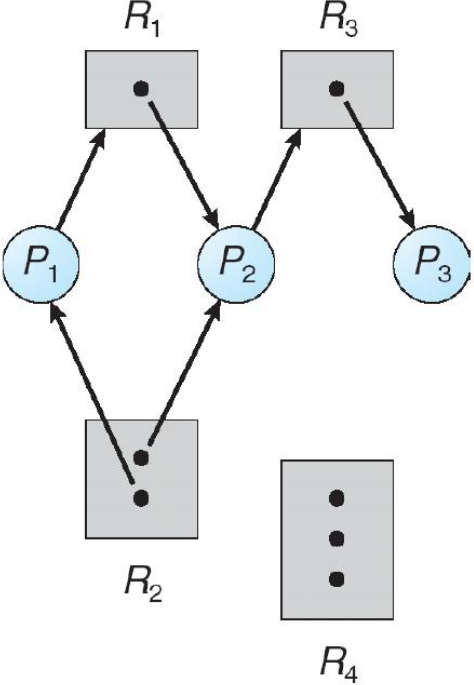
\includegraphics[width=0.15\textwidth]{ResourceAllocationGraph}\end{figure}
\end{items}

\paragraph{Deadlocks --- detection}
\begin{items}
  \item \textbf{principle}: allow system to enter deadlock $ \to $ detection $ \to $ recovery scheme
  \item \textbf{wait-for graph} (WFG): \\*
    $ - $ \emph{processes} = nodes \\*
    $ - $ \emph{wait-for relationship} = edges
  \item periodically invoke algorithm searching for cycle in graph \\*
    $ \leadsto $ cycle exists $ \to $ deadlock exists
\end{items}
\begin{figure}[H]\centering\label{WaitForGraph}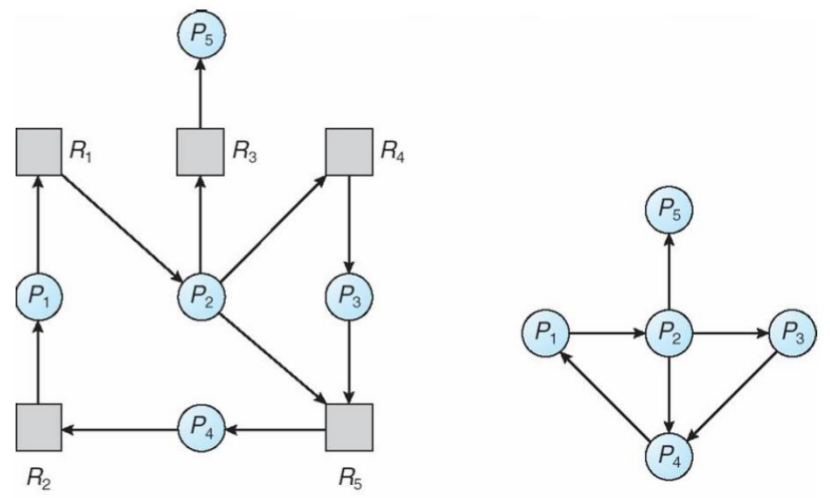
\includegraphics[width=0.33\textwidth]{WaitForGraph}\end{figure}

\paragraph{Deadlocks --- recovery}
\begin{items}
  \item \textbf{process termination}: \\*
    $ - $ \emph{all}: abort all deadlocked processes \\*
    $ - $ \emph{selective}: abort one process at a time until deadlock is eliminated
  \item \textbf{termination order}: in which order should processes be aborted? \\*
    $ - $ process priority \\*
    $ - $ how long already computed? how much longer for completion? \\*
    $ - $ amount of resources used \\*
    $ - $ amount of resources needed for completion \\*
    $ - $ how many processes will need to be terminated \\*
    $ - $ interactive or batch?
  \item \textbf{resource preemption}: \\*
    $ - $ \emph{victim selection}: minimize cost \\*
    $ - $ \emph{rollback}: perform periodic snapshots, abort process to preempt resources $ \to $ restart from last \\* \phantom{$ - $} \phantom{$ \cdot $} safe state \\*
    $ - $ \emph{starvation}: same process may always be picked as victim $ \leadsto $ include rollback count in cost factor
\end{items}

\begin{summary}
  \begin{items}
    \item \textbf{classical synchronization problems}: model synchronization problems occurring in reality \\*
      $ - $ \emph{producer-consumer}: shared use of buffers/queues \\*
      $ - $ \emph{reader-writer}: shared access to data structures \\*
      $ - $ \emph{dining philosophers}: competition for limited resources
    \item such synchronization problems occur very often when programming operating systems
    \item \textbf{parallelism}: introduced by multiple processors + multiprogramming, needs to be considered carefully when writing OS
  \end{items}
\end{summary}